\subsection{Existence of Drawings}
\label{subsect:application-existence-of-drawings}

\begin{frame}
  \frametitle{\insertsubsection}
  \begin{itemize}
    \item Circles are determined by three distinct points
    \item Necessary condition: ${\abs{V(P_i) \cap V(P_j)} \leq 2 \quad \forall i \neq j}$ \begin{itemize}
      \item Condition is not sufficient!
    \end{itemize}
  \end{itemize}
  \begin{figure}
    \includegraphics[height=3cm]{Resources/Arrangement-of-Pseudocircles}
    \quad
    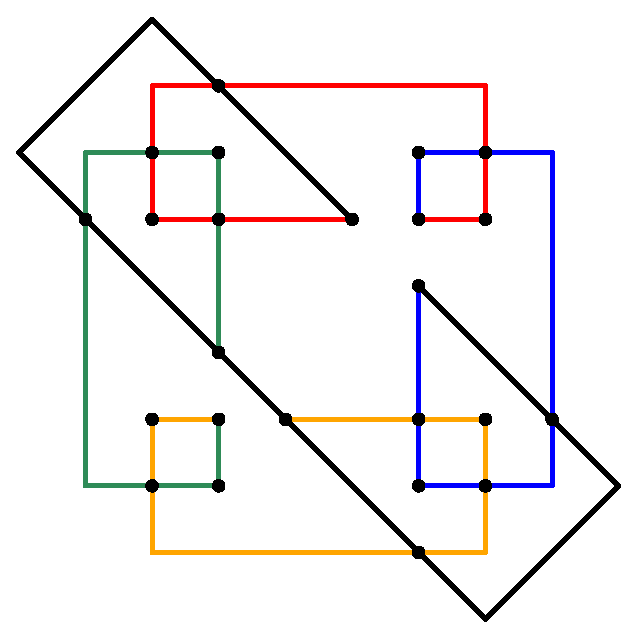
\includegraphics[height=3cm]{Resources/Arrangement-of-Pseudoarcs}
    \caption{An arrangement of pseudocircles that is not circleable (left) and a derived arrangement of pseudo circular arcs (right).}
  \end{figure}
\end{frame}

\begin{frame}
  \frametitle{\insertsubsection}
  \begin{itemize}
    \item Greedily realizable sequence of paths ${\Pi}$ \begin{itemize}
      \item Ordered sequence of edge-disjoint paths ${\Pi = (P_1, \ldots, P_k)}$
      \item ${V_\text{int}(P_i) \cap V(P_1 \cup \ldots \cup P_{i-1}) \stackrel{}{=} \varnothing, \quad i = 2 \ldots k}$
      \item Permits drawing with circular arcs using greedy algorithm
    \end{itemize}
  \end{itemize}
\end{frame}

\begin{frame}
  \frametitle{\insertsubsection}
  \begin{itemize}
    \item Greedily realizable sequence of paths ${\Pi}$ \begin{itemize}
      \item Ordered sequence of edge-disjoint paths ${\Pi = (P_1, \ldots, P_k)}$
      \item ${V_\text{int}(P_i) \cap V(P_1 \cup \ldots \cup P_{i-1}) \stackrel{}{=} \varnothing, \quad i = 2 \ldots k}$
      \item Permits drawing with circular arcs using greedy algorithm
    \end{itemize}
  \end{itemize}
  \begin{figure}
    \includegraphics<1>[height=4cm]{Resources/GreedyRealization-01}
    \includegraphics<2>[height=4cm]{Resources/GreedyRealization-02}
    \includegraphics<3>[height=4cm]{Resources/GreedyRealization-03}
    \includegraphics<4>[height=4cm]{Resources/GreedyRealization-04}
    \includegraphics<5>[height=4cm]{Resources/GreedyRealization-05}
    \includegraphics<6>[height=4cm]{Resources/GreedyRealization-06}
    \includegraphics<7>[height=4cm]{Resources/GreedyRealization-07}
    \includegraphics<8>[height=4cm]{Resources/GreedyRealization-08}
    \includegraphics<9>[height=4cm]{Resources/GreedyRealization-09}
    \includegraphics<10>[height=4cm]{Resources/GreedyRealization-10}
    \includegraphics<11>[height=4cm]{Resources/GreedyRealization-11}
    \caption{Greedy drawing of ${\Pi = ( \textit{abcde}, \textit{bfghd}, \textit{gijkl}, \textit{jmc} )}$}
  \end{figure}
\end{frame}

\begin{frame}
  \frametitle{\insertsubsection}
  \begin{itemize}
    \item Greedily realizable sequence of paths ${\Pi}$ \begin{itemize}
      \item Ordered sequence of edge-disjoint paths ${\Pi = (P_1, \ldots, P_k)}$
      \item ${V_\text{int}(P_i) \cap V(P_1 \cup \ldots \cup P_{i-1}) \stackrel{}{=} \varnothing, \quad i = 2 \ldots k}$
      \item Permits drawing with circular arcs using greedy algorithm
    \end{itemize}
    \item Characterization of vertices with respect to ${\Pi}$ \begin{itemize}
      \item Constrained vertices ${V_\text{c}(\Pi)}$: first appear as a path's internal vertex
      \item Unconstrained vertices ${V_\text{u}(\Pi)}$: first appear as a path's endpoint
    \end{itemize}
  \end{itemize}
\end{frame}
